\documentclass[10pt,a4paper,twocolumn]{article}
% Shared journal-style layout for main.tex and supplement.tex (compiled with tectonic by scripts/build_paper.py).
% Each document sets its own \documentclass and \geometry before and after % Shared journal-style layout for main.tex and supplement.tex (compiled with tectonic by scripts/build_paper.py).
% Each document sets its own \documentclass and \geometry before and after % Shared journal-style layout for main.tex and supplement.tex (compiled with tectonic by scripts/build_paper.py).
% Each document sets its own \documentclass and \geometry before and after \input{preamble}.
\usepackage{geometry}
\usepackage{fontspec}
\setmainfont{Charter}
\setsansfont{Helvetica Neue}[BoldFont={Helvetica Neue Bold}, ItalicFont={Helvetica Neue Italic},
  BoldItalicFont={Helvetica Neue Bold Italic}]
\usepackage{microtype}
\usepackage[table]{xcolor}
\usepackage{booktabs,tabularx,graphicx,array,makecell,longtable}
\usepackage{float}
\usepackage{enumitem}
\usepackage{etoolbox}
\usepackage{tikz}
\usetikzlibrary{positioning,calc}
\usepackage{titlesec}
\usepackage{fancyhdr}
\usepackage[numbers,sort&compress]{natbib}
\usepackage{caption}
\usepackage{hyperref}
\usepackage{xurl}

\definecolor{accent}{HTML}{1B4F72}
\definecolor{accentlight}{HTML}{EAF1F7}
\definecolor{tablehead}{HTML}{DCE7F1}
\hypersetup{colorlinks=true, linkcolor=accent, citecolor=accent, urlcolor=accent}
\urlstyle{same}

% Text
\setlength{\parindent}{1em}
\setlength{\parskip}{0pt}
\setlist{nosep,leftmargin=1.2em}
\titleformat{\section}{\sffamily\bfseries\large\color{accent}}{}{0pt}{}
\titleformat{\subsection}{\sffamily\bfseries\normalsize}{}{0pt}{}
\titlespacing*{\section}{0pt}{1.1em}{0.35em}
\titlespacing*{\subsection}{0pt}{0.7em}{0.15em}
\newcommand{\abshead}[1]{{\sffamily\bfseries\footnotesize\color{accent}\MakeUppercase{#1}}\enspace}

% Floats: sans-serif tables with a shaded header row, captions above tables
\captionsetup{font={footnotesize,sf}, labelfont={bf}, labelsep=period, justification=raggedright,
  singlelinecheck=false}
\captionsetup[table]{position=top, skip=4pt}
\AtBeginEnvironment{table}{\sffamily}
\AtBeginEnvironment{table*}{\sffamily}
\AtBeginEnvironment{longtable}{\sffamily}
\setlength{\aboverulesep}{0pt}
\setlength{\belowrulesep}{0pt}
\setlength{\extrarowheight}{1.6pt}
\arrayrulecolor{accent}
\setlength{\textfloatsep}{12pt plus 2pt minus 2pt}
\setlength{\dbltextfloatsep}{12pt plus 2pt minus 2pt}

% References
\renewcommand{\refname}{References}
\renewcommand{\bibfont}{\footnotesize}
\setlength{\bibsep}{1.2pt}

% Running heads and feet
\newcommand{\shorttitle}{Predicting prostate cancer treatment delays of more than 90 days}
\newcommand{\docversion}{Version 1, 14 September 2026}
\newcommand{\doclabel}{Preprint}
\newcommand{\footline}{\sffamily\scriptsize\textcolor{black!55}{\docversion}}
\fancypagestyle{journal}{%
  \fancyhf{}%
  \fancyhead[L]{\sffamily\scriptsize\textcolor{accent}{\bfseries\MakeUppercase{\doclabel}}\quad
    \textcolor{black!65}{\shorttitle}}%
  \fancyhead[R]{\sffamily\scriptsize\textcolor{black!65}{Hinge}}%
  \fancyfoot[L]{\footline}%
  \fancyfoot[R]{\sffamily\scriptsize\bfseries\thepage}%
  \renewcommand{\headrulewidth}{0.5pt}%
  \renewcommand{\headrule}{{\color{accent}\hrule height 0.5pt width \headwidth \vskip -0.5pt}}}
\fancypagestyle{firstpage}{%
  \fancyhf{}%
  \fancyfoot[L]{\footline}%
  \fancyfoot[R]{\sffamily\scriptsize\bfseries\thepage}%
  \renewcommand{\headrulewidth}{0pt}%
  \renewcommand{\headrule}{}}
\pagestyle{journal}

% Coloured band across the top of the first page
\newcommand{\topband}[2]{\noindent\colorbox{accent}{\parbox{\dimexpr\textwidth-2\fboxsep}{%
  \sffamily\footnotesize\bfseries\color{white}\strut #1\hfill #2}}}
.
\usepackage{geometry}
\usepackage{fontspec}
\setmainfont{Charter}
\setsansfont{Helvetica Neue}[BoldFont={Helvetica Neue Bold}, ItalicFont={Helvetica Neue Italic},
  BoldItalicFont={Helvetica Neue Bold Italic}]
\usepackage{microtype}
\usepackage[table]{xcolor}
\usepackage{booktabs,tabularx,graphicx,array,makecell,longtable}
\usepackage{float}
\usepackage{enumitem}
\usepackage{etoolbox}
\usepackage{tikz}
\usetikzlibrary{positioning,calc}
\usepackage{titlesec}
\usepackage{fancyhdr}
\usepackage[numbers,sort&compress]{natbib}
\usepackage{caption}
\usepackage{hyperref}
\usepackage{xurl}

\definecolor{accent}{HTML}{1B4F72}
\definecolor{accentlight}{HTML}{EAF1F7}
\definecolor{tablehead}{HTML}{DCE7F1}
\hypersetup{colorlinks=true, linkcolor=accent, citecolor=accent, urlcolor=accent}
\urlstyle{same}

% Text
\setlength{\parindent}{1em}
\setlength{\parskip}{0pt}
\setlist{nosep,leftmargin=1.2em}
\titleformat{\section}{\sffamily\bfseries\large\color{accent}}{}{0pt}{}
\titleformat{\subsection}{\sffamily\bfseries\normalsize}{}{0pt}{}
\titlespacing*{\section}{0pt}{1.1em}{0.35em}
\titlespacing*{\subsection}{0pt}{0.7em}{0.15em}
\newcommand{\abshead}[1]{{\sffamily\bfseries\footnotesize\color{accent}\MakeUppercase{#1}}\enspace}

% Floats: sans-serif tables with a shaded header row, captions above tables
\captionsetup{font={footnotesize,sf}, labelfont={bf}, labelsep=period, justification=raggedright,
  singlelinecheck=false}
\captionsetup[table]{position=top, skip=4pt}
\AtBeginEnvironment{table}{\sffamily}
\AtBeginEnvironment{table*}{\sffamily}
\AtBeginEnvironment{longtable}{\sffamily}
\setlength{\aboverulesep}{0pt}
\setlength{\belowrulesep}{0pt}
\setlength{\extrarowheight}{1.6pt}
\arrayrulecolor{accent}
\setlength{\textfloatsep}{12pt plus 2pt minus 2pt}
\setlength{\dbltextfloatsep}{12pt plus 2pt minus 2pt}

% References
\renewcommand{\refname}{References}
\renewcommand{\bibfont}{\footnotesize}
\setlength{\bibsep}{1.2pt}

% Running heads and feet
\newcommand{\shorttitle}{Predicting prostate cancer treatment delays of more than 90 days}
\newcommand{\docversion}{Version 1, 14 September 2026}
\newcommand{\doclabel}{Preprint}
\newcommand{\footline}{\sffamily\scriptsize\textcolor{black!55}{\docversion}}
\fancypagestyle{journal}{%
  \fancyhf{}%
  \fancyhead[L]{\sffamily\scriptsize\textcolor{accent}{\bfseries\MakeUppercase{\doclabel}}\quad
    \textcolor{black!65}{\shorttitle}}%
  \fancyhead[R]{\sffamily\scriptsize\textcolor{black!65}{Hinge}}%
  \fancyfoot[L]{\footline}%
  \fancyfoot[R]{\sffamily\scriptsize\bfseries\thepage}%
  \renewcommand{\headrulewidth}{0.5pt}%
  \renewcommand{\headrule}{{\color{accent}\hrule height 0.5pt width \headwidth \vskip -0.5pt}}}
\fancypagestyle{firstpage}{%
  \fancyhf{}%
  \fancyfoot[L]{\footline}%
  \fancyfoot[R]{\sffamily\scriptsize\bfseries\thepage}%
  \renewcommand{\headrulewidth}{0pt}%
  \renewcommand{\headrule}{}}
\pagestyle{journal}

% Coloured band across the top of the first page
\newcommand{\topband}[2]{\noindent\colorbox{accent}{\parbox{\dimexpr\textwidth-2\fboxsep}{%
  \sffamily\footnotesize\bfseries\color{white}\strut #1\hfill #2}}}
.
\usepackage{geometry}
\usepackage{fontspec}
\setmainfont{Charter}
\setsansfont{Helvetica Neue}[BoldFont={Helvetica Neue Bold}, ItalicFont={Helvetica Neue Italic},
  BoldItalicFont={Helvetica Neue Bold Italic}]
\usepackage{microtype}
\usepackage[table]{xcolor}
\usepackage{booktabs,tabularx,graphicx,array,makecell,longtable}
\usepackage{float}
\usepackage{enumitem}
\usepackage{etoolbox}
\usepackage{tikz}
\usetikzlibrary{positioning,calc}
\usepackage{titlesec}
\usepackage{fancyhdr}
\usepackage[numbers,sort&compress]{natbib}
\usepackage{caption}
\usepackage{hyperref}
\usepackage{xurl}

\definecolor{accent}{HTML}{1B4F72}
\definecolor{accentlight}{HTML}{EAF1F7}
\definecolor{tablehead}{HTML}{DCE7F1}
\hypersetup{colorlinks=true, linkcolor=accent, citecolor=accent, urlcolor=accent}
\urlstyle{same}

% Text
\setlength{\parindent}{1em}
\setlength{\parskip}{0pt}
\setlist{nosep,leftmargin=1.2em}
\titleformat{\section}{\sffamily\bfseries\large\color{accent}}{}{0pt}{}
\titleformat{\subsection}{\sffamily\bfseries\normalsize}{}{0pt}{}
\titlespacing*{\section}{0pt}{1.1em}{0.35em}
\titlespacing*{\subsection}{0pt}{0.7em}{0.15em}
\newcommand{\abshead}[1]{{\sffamily\bfseries\footnotesize\color{accent}\MakeUppercase{#1}}\enspace}

% Floats: sans-serif tables with a shaded header row, captions above tables
\captionsetup{font={footnotesize,sf}, labelfont={bf}, labelsep=period, justification=raggedright,
  singlelinecheck=false}
\captionsetup[table]{position=top, skip=4pt}
\AtBeginEnvironment{table}{\sffamily}
\AtBeginEnvironment{table*}{\sffamily}
\AtBeginEnvironment{longtable}{\sffamily}
\setlength{\aboverulesep}{0pt}
\setlength{\belowrulesep}{0pt}
\setlength{\extrarowheight}{1.6pt}
\arrayrulecolor{accent}
\setlength{\textfloatsep}{12pt plus 2pt minus 2pt}
\setlength{\dbltextfloatsep}{12pt plus 2pt minus 2pt}

% References
\renewcommand{\refname}{References}
\renewcommand{\bibfont}{\footnotesize}
\setlength{\bibsep}{1.2pt}

% Running heads and feet
\newcommand{\shorttitle}{Predicting prostate cancer treatment delays of more than 90 days}
\newcommand{\docversion}{Version 1, 14 September 2026}
\newcommand{\doclabel}{Preprint}
\newcommand{\footline}{\sffamily\scriptsize\textcolor{black!55}{\docversion}}
\fancypagestyle{journal}{%
  \fancyhf{}%
  \fancyhead[L]{\sffamily\scriptsize\textcolor{accent}{\bfseries\MakeUppercase{\doclabel}}\quad
    \textcolor{black!65}{\shorttitle}}%
  \fancyhead[R]{\sffamily\scriptsize\textcolor{black!65}{Hinge}}%
  \fancyfoot[L]{\footline}%
  \fancyfoot[R]{\sffamily\scriptsize\bfseries\thepage}%
  \renewcommand{\headrulewidth}{0.5pt}%
  \renewcommand{\headrule}{{\color{accent}\hrule height 0.5pt width \headwidth \vskip -0.5pt}}}
\fancypagestyle{firstpage}{%
  \fancyhf{}%
  \fancyfoot[L]{\footline}%
  \fancyfoot[R]{\sffamily\scriptsize\bfseries\thepage}%
  \renewcommand{\headrulewidth}{0pt}%
  \renewcommand{\headrule}{}}
\pagestyle{journal}

% Coloured band across the top of the first page
\newcommand{\topband}[2]{\noindent\colorbox{accent}{\parbox{\dimexpr\textwidth-2\fboxsep}{%
  \sffamily\footnotesize\bfseries\color{white}\strut #1\hfill #2}}}

\geometry{top=21mm, bottom=22mm, left=17mm, right=17mm, columnsep=6.5mm, headsep=5mm, footskip=9mm}

\begin{document}

\twocolumn[{%
\thispagestyle{firstpage}
\topband{HEALTH SERVICES RESEARCH AND MACHINE LEARNING}{PREPRINT VERSION}

\vspace{12pt}
{\raggedright\sffamily\bfseries\fontsize{19}{23}\selectfont Predicting treatment delays of more than 90 days in prostate cancer: added value of county rurality, county income and marital status over clinical characteristics\par}
\vspace{5pt}
{\raggedright\sffamily\large\color{black!70} A machine learning cohort study of 330,827 men treated with surgery or radiotherapy in US SEER registries, 2010 to 2022\par}
\vspace{9pt}
{\raggedright\sffamily\bfseries Tanmay Hinge\par}
\vspace{9pt}
{\color{accent}\hrule height 0.8pt}
\vspace{9pt}
\noindent
\begin{minipage}[t]{0.645\textwidth}
\setlength{\parskip}{4pt}\small
{\sffamily\bfseries\normalsize\color{accent} Abstract\par}
%% abstract-start
\abshead{Background} It is unclear how much area and marital characteristics add to clinical information in predicting delayed prostate cancer treatment.

\abshead{Methods} In this retrospective cohort study of SEER 17 registry data, we included men aged 40 or over diagnosed 2010 to 2022 with localised or regional prostate cancer and recorded radical prostatectomy or radiotherapy. The outcome was first recorded treatment over 90 days after diagnosis. Penalised logistic regression and LightGBM were cross-fitted in ordered steps (year; clinical need; county rurality, county income and marital status; treatment type) within risk groups. The primary estimand was the out-of-fold log-loss skill added by the area and marital block.

\abshead{Results} Of 330,827 men, 39.7\% waited more than 90 days, rising from 36.0\% in 2010 to 52.3\% in 2022. Prediction was weak (AUC 0.592 to 0.663). The area and marital block added 0.62 percentage points of skill (95\% interval 0.39 to 0.87) with logistic regression and 0.99 (0.73 to 1.30) with LightGBM, and was stable across robustness checks. With the two models, standardised delay was 9.2 and 8.8 points lower in non-metropolitan counties not adjacent to a metropolitan area than in large metropolitan counties, and 6.7 and 5.9 points higher in never-married than married men (post hoc agreement rule; no intervals).

\abshead{Conclusions} Registry data predict little of who waits beyond 90 days. Area and marital characteristics add a small, consistent gain. Delay was more common in large metropolitan, higher-income counties, which is not evidence of better care elsewhere, because recorded treatment also differs by area.
%% abstract-end

{\sffamily\footnotesize\textbf{Keywords}\enspace prostate cancer; time to treatment; health services research; machine learning; health equity\par}
\end{minipage}\hfill
\begin{minipage}[t]{0.325\textwidth}
\vspace{0pt}
\colorbox{accentlight}{\parbox{\dimexpr\linewidth-2\fboxsep}{\sffamily\footnotesize\setlength{\parskip}{4pt}\raggedright
\vspace{2pt}{\bfseries\color{accent}KEY POINTS}\par
\textbf{Question}\enspace How much do county rurality, county income and marital status add to clinical information in predicting a wait of more than 90 days for radical prostatectomy or radiotherapy?\par
\textbf{Findings}\enspace In this cohort study of 330,827 US men, registry information predicted delay weakly (AUC 0.592 to 0.663). Area and marital characteristics added 0.62 (logistic regression) and 0.99 (LightGBM) percentage points of log-loss skill in all men, with 95\% intervals above 0 in every risk group.\par
\textbf{Meaning}\enspace Who waits beyond 90 days is mostly not explained by registry data. County and marital characteristics carry a small, consistent signal whose causes these data cannot identify.\par\vspace{2pt}}}

\vspace{6pt}
{\sffamily\scriptsize\raggedright\setlength{\parskip}{4pt}\color{black!80}
\textbf{Corresponding author}\\Tanmay Hinge, \href{mailto:hingetanmay@gmail.com}{hingetanmay@gmail.com}\par
\textbf{Preprint status}\\\docversion.\par
\textbf{Data}\\SEER Research Data, 17 registries, November 2025 submission.\par
\textbf{Code and protocol}\\\href{https://github.com/tanmayhinge/seer-prostate}{github.com/tanmayhinge/seer-prostate}\par
\textbf{Supplementary material}\\Tables S1 to S11 and Figures S1 to S3.\par}
\end{minipage}

\vspace{9pt}
{\color{accent}\hrule height 0.8pt}
\vspace{14pt}
}]

%% main-text-start
\section{Introduction}

Time from diagnosis to first treatment is a widely used measure of the timeliness of cancer care. In the US National Cancer Database, the median time to first treatment for six early-stage cancers rose from 21 to 29 days between 2004 and 2013, and care at an academic centre was among the factors associated with longer intervals~\cite{khorana2019}. Prostate cancer intervals are longer still. The median was 79 days (interquartile range 55 to 117) in the same database for 2004 to 2015~\cite{cone2020}, and the mean in SEER was 82.75 days in 2021~\cite{abdelrahman2026}.

Several studies describe who waits longer. In SEER-Medicare data, time to definitive treatment was longer for African American than for White men with localised prostate cancer, and longer in high-risk than in low-risk disease~\cite{stokes2013}. Across four cancers in SEER, lower-income and non-metropolitan patients had shorter intervals~\cite{divanna2025}. In the Tennessee cancer registry, men living in rural Appalachian counties had lower odds of waiting more than 90 days for prostate cancer treatment (odds ratio 0.83, 95\% CI 0.78 to 0.89)~\cite{montielishino2021}. Care at an accredited hospital was associated with a longer median interval in low-income but not high-income counties~\cite{semprini2026}. Unadjusted comparisons can mislead: in SEER, all-cause mortality was lower among patients with longer intervals~\cite{ang2025}, which is consistent with more aggressive disease being treated sooner.

These studies tell us which factors are associated with waiting. They do not tell us how much of the variation in waiting can be predicted from a man's clinical record, or how much his county's rurality and income and his marital status add to that. This kind of added predictive value has been measured for other prostate cancer outcomes~\cite{tagai2025,ajjawi2026}. In a PubMed search screened by one reviewer, we found no study that had measured it for time to treatment. Measuring the gain on patients a model has not seen avoids deciding in advance which direction a difference should run. Fitting a flexible model, gradient boosting~\cite{ke2017}, alongside penalised regression also checks that a gain is not simply the product of a clinical model that is too simple.

We set out to measure how much county rurality, county income and marital status add to clinical information when predicting whether a man treated with radical prostatectomy or radiotherapy waits more than 90 days. We did this within clinical risk groups, and expressed the result as standardised percentages and an income concentration index.

\section{Methods}

\subsection{Data and cohort}
We used the SEER Research Data, 17 registries, November 2025 submission, linked to county attributes~\cite{seer2025}. A case listing selected by site (prostate) and year of diagnosis gave 793,214 tumour records. Exclusions were applied in a pre-specified order (Figure~\ref{fig:flow}): first primary cancer; localised or regional Combined Summary Stage; not a death certificate or autopsy case; aged 40 or over; diagnosed 2010 to 2022; first course including radical prostatectomy (surgery codes 50, 70 or 80, or A500, A700 or A800 from 2023) or radiotherapy~\cite{seermanual}; a recorded or top-coded interval; and an interval above 0 days. The SEER coding manual instructs that treatment is coded as not done when the physician opts for active surveillance or watchful waiting, so men managed this way are not in the cohort~\cite{seermanual}.

\begin{figure}[t]
\centering
\begin{tikzpicture}[>=latex, font=\footnotesize,
  cohortbox/.style={draw, align=center, text width=6.2cm, inner sep=3pt},
  exclusionbox/.style={draw, align=left, text width=6.0cm, inner sep=3pt, fill=black!4}]
\node[cohortbox] (s0) {All prostate cancer records\\n = 793,214};
\node[cohortbox, below=6mm of s0] (s1) {First primary cancer\\n = 710,343};
\draw[->] (s0) -- (s1);
\node[exclusionbox, anchor=west] (e1) at ($(s0.south)!0.5!(s1.north) + (3.9cm,0)$) {Not the first primary cancer\\n = 82,871};
\draw[->] ($(s0.south)!0.5!(s1.north)$) -- (e1.west);
\node[cohortbox, below=6mm of s1] (s2) {Localised or regional stage\\n = 608,441};
\draw[->] (s1) -- (s2);
\node[exclusionbox, anchor=west] (e2) at ($(s1.south)!0.5!(s2.north) + (3.9cm,0)$) {Not localised or regional stage\\n = 101,902};
\draw[->] ($(s1.south)!0.5!(s2.north)$) -- (e2.west);
\node[cohortbox, below=6mm of s2] (s3) {Not death certificate or autopsy only\\n = 608,375};
\draw[->] (s2) -- (s3);
\node[exclusionbox, anchor=west] (e3) at ($(s2.south)!0.5!(s3.north) + (3.9cm,0)$) {Death certificate or autopsy only\\n = 66};
\draw[->] ($(s2.south)!0.5!(s3.north)$) -- (e3.west);
\node[cohortbox, below=6mm of s3] (s4) {Aged 40 or over\\n = 608,133};
\draw[->] (s3) -- (s4);
\node[exclusionbox, anchor=west] (e4) at ($(s3.south)!0.5!(s4.north) + (3.9cm,0)$) {Not aged 40 or over\\n = 242};
\draw[->] ($(s3.south)!0.5!(s4.north)$) -- (e4.west);
\node[cohortbox, below=6mm of s4] (s5) {Diagnosed 2010 to 2022\\n = 557,683};
\draw[->] (s4) -- (s5);
\node[exclusionbox, anchor=west] (e5) at ($(s4.south)!0.5!(s5.north) + (3.9cm,0)$) {Not diagnosed 2010 to 2022\\n = 50,450};
\draw[->] ($(s4.south)!0.5!(s5.north)$) -- (e5.west);
\node[cohortbox, below=6mm of s5] (s6) {Radical prostatectomy or radiotherapy recorded\\n = 355,581};
\draw[->] (s5) -- (s6);
\node[exclusionbox, anchor=west] (e6) at ($(s5.south)!0.5!(s6.north) + (3.9cm,0)$) {No radical prostatectomy or radiotherapy\\n = 202,102};
\draw[->] ($(s5.south)!0.5!(s6.north)$) -- (e6.west);
\node[cohortbox, below=6mm of s6] (s7) {Interval recorded or top-coded\\n = 338,580};
\draw[->] (s6) -- (s7);
\node[exclusionbox, anchor=west] (e7) at ($(s6.south)!0.5!(s7.north) + (3.9cm,0)$) {No recorded interval\\n = 17,001};
\draw[->] ($(s6.south)!0.5!(s7.north)$) -- (e7.west);
\node[cohortbox, below=6mm of s7] (s8) {\textbf{Primary cohort: interval above 0 days}\\n = 330,827};
\draw[->] (s7) -- (s8);
\node[exclusionbox, anchor=west] (e8) at ($(s7.south)!0.5!(s8.north) + (3.9cm,0)$) {Interval of 0 days\\n = 7,753};
\draw[->] ($(s7.south)!0.5!(s8.north)$) -- (e8.west);
\end{tikzpicture}

\caption{Inclusion flow for the primary cohort. Boxes give the number of records remaining after each step, in protocol order; shaded boxes give the number excluded at that step.}
\label{fig:flow}
\end{figure}

\subsection{Outcome and risk groups}
The outcome used SEER's time from diagnosis to treatment in days. This interval ends at the first treatment of any kind, so hormone therapy, which this export does not record, can end it before surgery or radiotherapy. The primary outcome was a wait of more than 90 days. This threshold has been used in US registry research~\cite{montielishino2021} and matches the Australian optimal care pathway recommendation that surgery or radiotherapy begin within 3 months of diagnosis~\cite{ocp2021}. Intervals top-coded at 731 days or more counted as delayed, and thresholds of 60, 120 and 180 days were sensitivity analyses. Risk groups were high (regional stage, clinical Gleason score 8 to 10, or PSA above 20 ng/ml), unknown (otherwise, Gleason score or PSA missing), intermediate (Gleason score 7 or PSA 10 to 20 ng/ml) and low (Gleason score 6 or lower and PSA below 10 ng/ml). Summary stage can incorporate pathology for surgically treated men.

\subsection{Ordered feature steps}
Step 0 contained year of diagnosis and a 2020 indicator. Step 1 added clinical need: stage category, clinical Gleason score, log PSA (with missing and top-code indicators) and age band. Step 2 added the area and marital block: marital status (7 categories), county Rural-Urban Continuum Code (5 levels plus unknown) and county median household income (16 bands, entered as a rank). Rurality and income describe the county, not the man. Because the export has no registry identifier, this block may also pick up differences in registry practice. Step 3 added treatment type. It came last because area and marital characteristics can influence which treatment a man receives.

\subsection{Models and validation}
Penalised logistic regression used an L2 penalty, median imputation, standardisation and pairwise products of the clinical features~\cite{pedregosa2011}. LightGBM handled missing values internally~\cite{ke2017}. Every performance measure came from out-of-fold predictions, using 5-fold stratified cross-fitting within each risk group and in all men. Hyperparameters were tuned by 3-fold cross-validated log-loss on up to 50,000 men at step 3 and reused at every step. The main performance measure was log-loss skill, the proportional reduction in log-loss compared with the step 0 model, and the primary estimand was the skill added between steps 1 and 2. We also report AUC and calibration slope. Men in the same county share its rurality and income, but the export has no county identifier. We therefore used a cluster bootstrap over the 79 cells formed by rurality and income band (500 resamples of the out-of-fold predictions). Models were not refitted within the bootstrap, so the intervals leave out model-fitting variability.

\subsection{Standardised percentages and income concentration}
Standardised percentages came from g-computation with the step 2 model. Each man kept his own clinical features and year of diagnosis, while his area and marital features were set to a chosen profile. The reference profile was a married man living in a metropolitan area of 1 million or more, at the 83.33\% quantile of county income rank. Rurality and income are closely linked, so area profiles set both together, using the median income band of men living in each type of area. The two model types disagreed in a development run. After seeing this, we adopted a post hoc rule that a contrast is treated as meaningful only when both models agree on a difference of 3 percentage points or more in the same direction, and we dropped the planned intervals for these contrasts, also post hoc. Income inequality in delay was summarised with the Erreygers-corrected concentration index~\cite{erreygers2009}, ranking men by county income (tied men share the average rank). The index is crude and does not separate income from rurality.

\subsection{Robustness, selection and secondary outcome}
Ten sensitivity scenarios each changed one setting: thresholds of 60, 120 and 180 days; risk groups from Gleason score and PSA only; prostatectomy without radiotherapy; excluding 2020; including 2023; including 0-day intervals; one primary cancer only; and excluding prostatectomy not otherwise specified. A later protocol amendment (version 1.9) added six further checks, each specified before it was run: tuning at each step, 10 fold-assignment seeds, clustering by county income band alone, a clinical block without stage, year as categories, and the concentration index by diagnosis period. For treated men without a recorded interval, we bounded the percentage delayed under extreme assumptions and reweighted by the inverse probability of having an interval. The secondary outcome was any record of radical prostatectomy or radiotherapy among intermediate- and high-risk men. SEER captures treatment incompletely (radiation therapy sensitivity 80\% against Medicare claims, pooled across cancer sites)~\cite{noone2016}, so a missing record does not prove a man was untreated.

\subsection{Protocol, reporting and disclosure}
We wrote the protocol and committed it to version control before building the cohort or fitting any model. It was amended 13 times. Three amendments followed a look at results and are marked as such, and the log and commit history are public (analyses fixed at commit c1b6fd7). The study was not registered. Reporting follows STROBE~\cite{strobe2007}, RECORD~\cite{record2015} and TRIPOD+AI~\cite{tripodai2024} (Supplementary Tables S10 and S11). The models are measurement tools, not clinical tools. As the SEER Research Data Use Agreement requires, statistics based on 1 to 4 men are suppressed. Analyses used Python 3.13, scikit-learn 1.9.1 and LightGBM 4.7.0 (seed 20260913).

\section{Results}

\subsection{Cohort and delay}
Of 793,214 records, 330,827 men met all criteria (Figure~\ref{fig:flow}; Table~\ref{tab:cohort}). The median wait from diagnosis to treatment was 77 days (interquartile range 52 to 116), and 131,326 men (39.7\%) waited more than 90 days. The share waiting that long rose from 36.0\% in 2010 to 52.3\% in 2022.

Low-risk men waited longest: 47.9\% waited more than 90 days, compared with 42.8\% of intermediate-risk and 32.8\% of high-risk men. For these men a longer wait is not necessarily worse care. In every risk group, delay was more common in the largest metropolitan areas than in non-metropolitan counties not adjacent to one (low risk 50.7\% against 39.0\%; high risk 35.7\% against 26.0\%; Supplementary Figure S1). It was also more common among never-married than married men (high risk 40.0\% against 30.9\%). Rurality and income were closely linked. Almost half (45.6\%) of men in non-metropolitan counties not adjacent to a metropolitan area lived in the lowest county income quartile, compared with 1.1\% of men in the largest metropolitan areas.

\begin{table*}[tbp]
\centering\sffamily
\footnotesize
\setlength{\tabcolsep}{6pt}
\caption{Characteristics of the 330,827 men in the cohort, by county rurality}
\label{tab:cohort}
\begin{tabular}{@{}l*{6}{r}@{}}
\toprule
\rowcolor{tablehead}Characteristic & Overall & \makecell[r]{Metro,\\1 million\\or more} & \makecell[r]{Metro,\\250,000 to\\1 million} & \makecell[r]{Metro,\\under\\250,000} & \makecell[r]{Nonmetro,\\adjacent\\to metro} & \makecell[r]{Nonmetro,\\not adjacent\\to metro} \\
\midrule
Men, n & 330,827 & 194,681 & 72,150 & 26,092 & 23,360 & 14,385 \\
\textit{Risk group} &  &  &  &  &  &  \\
\quad Low & 17.4 & 17.6 & 16.5 & 18.3 & 17.1 & 17.5 \\
\quad Intermediate & 38.6 & 38.6 & 39.0 & 38.6 & 37.8 & 37.2 \\
\quad High & 39.6 & 38.9 & 40.6 & 38.8 & 41.0 & 41.8 \\
\quad Unknown & 4.5 & 4.9 & 3.8 & 4.3 & 4.1 & 3.5 \\
\textit{Summary stage} &  &  &  &  &  &  \\
\quad Localised & 77.5 & 77.7 & 76.7 & 78.7 & 77.4 & 77.9 \\
\quad Regional, direct extension & 18.7 & 18.4 & 19.6 & 18.2 & 19.3 & 18.8 \\
\quad Regional, lymph nodes & 3.7 & 3.9 & 3.7 & 3.1 & 3.2 & 3.3 \\
\textit{Marital status} &  &  &  &  &  &  \\
\quad Married & 70.3 & 69.6 & 71.7 & 69.5 & 71.5 & 71.7 \\
\quad Never married & 11.1 & 11.6 & 10.8 & 10.5 & 10.1 & $<$5 \\
\quad Divorced & 6.7 & 6.3 & 6.8 & 7.4 & 7.6 & 7.8 \\
\quad Widowed & 3.0 & 2.7 & 3.1 & 3.5 & 3.7 & 3.8 \\
\quad Unknown & 7.8 & 8.5 & 6.4 & 7.9 & 6.2 & 6.8 \\
\textit{County income quartile} &  &  &  &  &  &  \\
\quad Q1 (lowest) & 8.0 & 1.1 & 5.0 & 20.2 & 37.7 & 45.6 \\
\quad Q2 & 24.1 & 12.4 & 32.5 & 58.4 & 45.1 & 44.4 \\
\quad Q3 & 35.1 & 42.7 & 33.9 & 18.0 & 11.0 & 8.9 \\
\quad Q4 (highest) & 32.8 & 43.7 & 28.6 & 3.3 & 6.2 & 1.1 \\
\textit{First-course treatment} &  &  &  &  &  &  \\
\quad Radical prostatectomy & 48.2 & 48.3 & 48.9 & 49.0 & 45.7 & 46.4 \\
\quad Radiotherapy & 47.9 & 47.9 & 46.9 & 47.2 & 50.8 & 50.1 \\
\quad Both & 3.9 & 3.8 & 4.2 & 3.8 & 3.5 & 3.5 \\
\textit{Days to first recorded treatment} &  &  &  &  &  &  \\
\quad Median & 77 & 81 & 76 & 71 & 70 & 68 \\
\quad Interquartile range & 52 to 116 & 55 to 121 & 50 to 112 & 48 to 106 & 46 to 105 & 43 to 103 \\
Waited more than 90 days & 39.7 & 42.5 & 37.6 & 34.2 & 33.2 & 32.2 \\
\bottomrule
\end{tabular}
\par\smallskip
\begin{minipage}{\linewidth}\scriptsize Values are the percentage of men in the column unless stated. Rurality is the county Rural-Urban Continuum Code at diagnosis; 159 men with unknown rurality are included in Overall only. Separated (0.8\%) and unmarried or domestic partner (0.4\%) men are not shown. $<$5: suppressed under the SEER Research Data Use Agreement, either because it rests on 1 to 4 men or because a total would reveal such a cell. County income quartiles are formed from 16 bands of county median household income.\end{minipage}
\end{table*}


\subsection{How much area and marital characteristics add}
Delay was hard to predict. At step 2, AUC ranged from 0.592 to 0.663 across risk groups and models, and log-loss skill from 0.76\% to 4.90\% (Table~\ref{tab:models}).

Clinical information helped mostly for high-risk men. With logistic regression it added 3.01 percentage points of skill in all men (95\% interval 2.69 to 3.38) and 3.53 in high-risk men, but only 0.14 (0.08 to 0.20) in low-risk men, whose clinical features vary little by definition.

Adding county rurality, county income and marital status improved prediction in every risk group, and every 95\% interval lay above 0 (Figure~\ref{fig:skill}). In all men the gain was 0.62 points (0.39 to 0.87) with logistic regression and 0.99 points (0.73 to 1.30) with LightGBM. In low-risk men, where clinical information added little, this block made up most of a small total: 82\% of the 0.76 points of step 2 skill with logistic regression, and 98\% of the 0.99 points with LightGBM. LightGBM predicted better than logistic regression in every risk group, but only by 0.23 to 0.90 points (no interval computed). Calibration slopes were 0.98 to 1.00 for logistic regression and 0.88 to 1.03 for LightGBM.

\begin{table*}[tbp]
\centering\sffamily
\footnotesize
\setlength{\tabcolsep}{5pt}
\caption{Predictive performance and skill added by clinical need and by area and marital characteristics, by risk group and model}
\label{tab:models}
\begin{tabular}{@{}llrrrrrr@{}}
\toprule
\rowcolor{tablehead}\makecell[l]{Risk group} & \makecell[l]{Model} & \makecell[r]{Men} & \makecell[r]{Skill at\\step 2 (\%)} & \makecell[r]{AUC at\\step 2} & \makecell[r]{Clinical need\\added (95\% interval)} & \makecell[r]{Area and marital\\added (95\% interval)} & \makecell[r]{Fold-seed\\range\textsuperscript{a}} \\
\midrule
All men & Logistic & 330,827 & 3.63 & 0.638 & 3.01 (2.69 to 3.38) & 0.62 (0.39 to 0.87) & 0.61 to 0.62 \\
 & LightGBM & 330,827 & 4.17 & 0.648 & 3.18 (2.85 to 3.54) & 0.99 (0.73 to 1.30) & 0.98 to 0.99 \\
Low & Logistic & 57,495 & 0.76 & 0.592 & 0.14 (0.08 to 0.20) & 0.62 (0.32 to 0.94) & 0.59 to 0.63 \\
 & LightGBM & 57,495 & 0.99 & 0.604 & 0.02 ($-$0.09 to 0.13) & 0.96 (0.67 to 1.28) & 0.95 to 1.01 \\
Intermediate & Logistic & 127,622 & 1.06 & 0.605 & 0.49 (0.41 to 0.56) & 0.56 (0.35 to 0.83) & 0.54 to 0.56 \\
 & LightGBM & 127,622 & 1.48 & 0.615 & 0.55 (0.44 to 0.65) & 0.93 (0.65 to 1.27) & 0.91 to 0.97 \\
High & Logistic & 130,893 & 4.39 & 0.654 & 3.53 (3.16 to 3.86) & 0.86 (0.60 to 1.15) & 0.85 to 0.86 \\
 & LightGBM & 130,893 & 4.90 & 0.663 & 3.72 (3.34 to 4.06) & 1.18 (0.90 to 1.56) & 1.16 to 1.20 \\
Unknown & Logistic & 14,817 & 1.07 & 0.610 & 0.65 (0.41 to 0.89) & 0.42 (0.08 to 0.80) & 0.32 to 0.48 \\
 & LightGBM & 14,817 & 1.96 & 0.629 & 0.59 (0.27 to 0.95) & 1.37 (0.80 to 2.19) & 1.22 to 1.43 \\
\bottomrule
\end{tabular}
\par\smallskip
\begin{minipage}{\linewidth}\scriptsize Skill is the percentage reduction in out-of-fold log-loss against the step 0 model (year of diagnosis only); added values are in percentage points. Intervals are 95\% cluster bootstrap intervals over 79 rurality by county income cells (500 resamples of out-of-fold predictions, no refitting), so they exclude model-fitting variability. \textsuperscript{a}Range of the area and marital increment over 10 fold assignments, from the post-review analysis with per-step tuning (protocol amendment 1.9). AUC: 0.5 is chance.\end{minipage}
\end{table*}


\begin{figure*}[t]
\centering
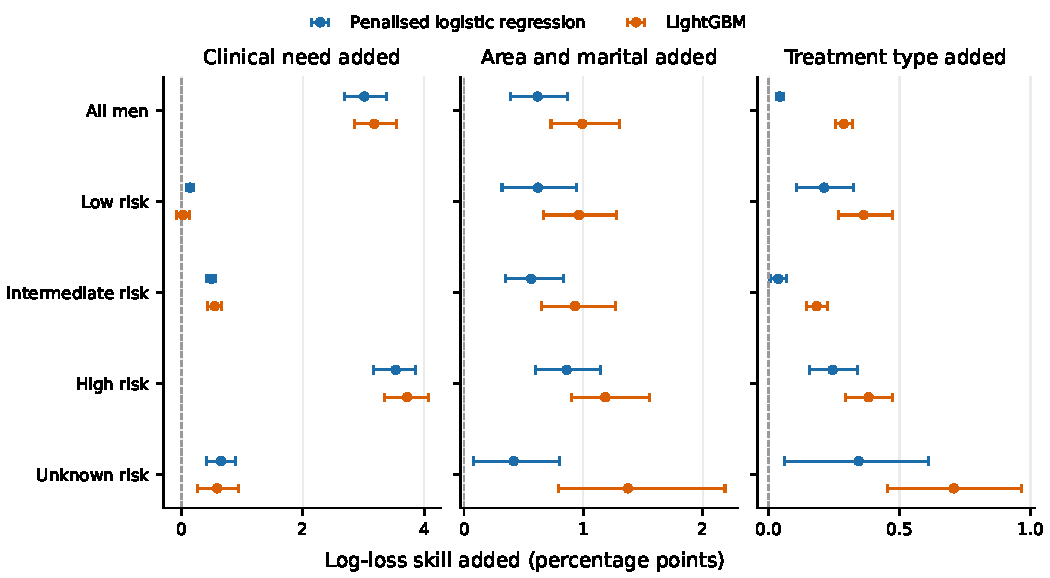
\includegraphics[width=0.86\textwidth]{../figures/figure3_skill_added.pdf}
\caption{Out-of-fold log-loss skill added by each block of features, in percentage points, by risk group and model type, with 95\% cluster bootstrap intervals (500 resamples, no refitting). The dashed line marks no added skill, and the x-axis scale differs between panels.}
\label{fig:skill}
\end{figure*}

\subsection{Standardised differences and income concentration}
With clinical features held as observed, men in non-metropolitan counties not adjacent to a metropolitan area were less likely to wait more than 90 days than men in the largest metropolitan areas, each area set to its typical county income. The difference was 9.2 percentage points with logistic regression and 8.8 with LightGBM in all men, and 7.2 to 14.2 points across risk groups (Figure~\ref{fig:area}a). Because this comparison moves rurality and income together, it cannot show which of the two carries the difference. Changing either alone gave the models conflicting answers: $-$8.7 points with logistic regression and $+$1.7 with LightGBM for rurality, and $-$0.9 and $-$8.7 points for income.

Never-married men were 6.7 points (logistic regression) and 5.9 points (LightGBM) more likely to wait than married men. Both models agreed on a difference of at least 3 points in every risk group except low risk, where the differences were 3.6 and 2.4 points (Supplementary Table S6). Across the whole cohort these characteristics moved the overall percentage very little: setting every man to the reference profile changed it by 1.1 and 1.6 points.

Crude delay was concentrated in higher-income counties (Erreygers index 0.062, 95\% interval 0.039 to 0.083; Figure~\ref{fig:area}b). The index was smaller within diagnosis periods: 0.059 in 2010 to 2014, 0.037 in 2015 to 2019 and 0.027 in 2020 to 2022 (Supplementary Table S7). Over the same years, the share of men living in the highest income quartile rose from 26.2\% to 41.0\%.

\begin{figure*}[t]
\centering
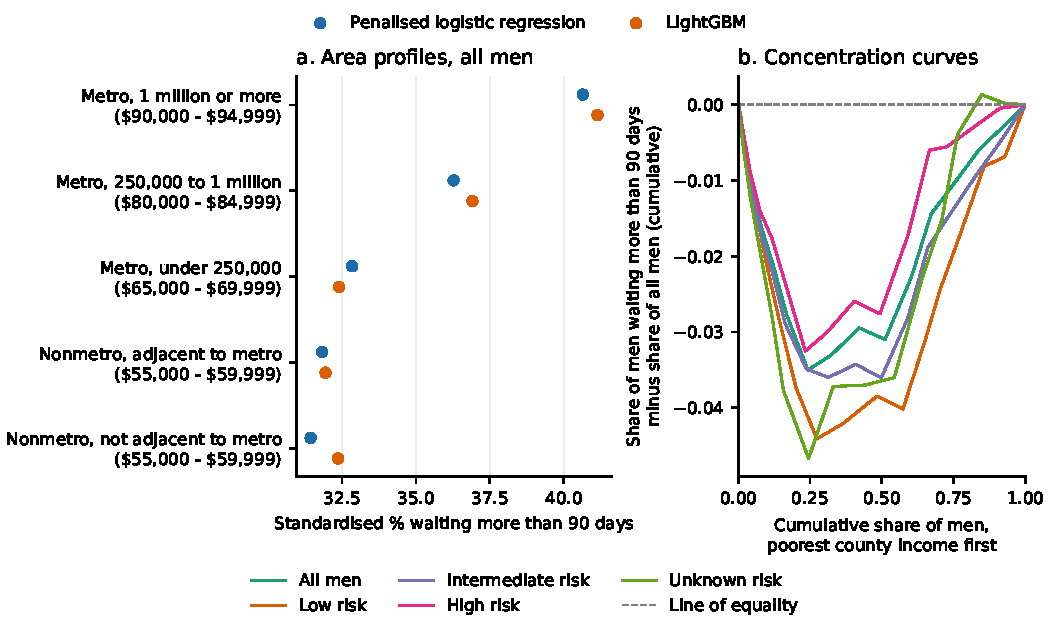
\includegraphics[width=0.86\textwidth]{../figures/figure4_area_and_income.pdf}
\caption{(a) Standardised percentage of all men waiting more than 90 days, with rurality and county income set together to each type of area at the median income band of men living there; each man keeps his own clinical features and year, and marital status is set to married. (b) Crude concentration curves of waiting more than 90 days by county income rank, shown as the difference from the line of equality; values below 0 mean delay is concentrated among men in higher-income counties. Neither panel separates income from rurality.}
\label{fig:area}
\end{figure*}

\subsection{Robustness, selection and secondary outcome}
The area and marital gain held up under the additional checks (Supplementary Tables S3 to S5). Tuning at each step left it unchanged. Across 10 different fold assignments it moved only between 0.61 and 0.62 points with logistic regression and between 0.98 and 0.99 with LightGBM in all men, and its smallest value stayed above 0 in every risk group. Its intervals also stayed above 0 when clustering by county income band alone. Across the ten sensitivity scenarios, the interval lay above 0 in 98 of 100 results. The area difference met the two-model rule in 9 of 10 scenarios, falling just short at a 180-day threshold ($-$2.96 and $-$3.20 points), and the marital difference met it in all 10.

There was one caveat. In low-risk and unknown-risk men, LightGBM's clinical model was weaker than logistic regression's (0.05 against 0.14 points, and 0.55 against 0.64), so its larger gain there may partly reflect a weaker starting point. With tuning at each step, logistic regression also chose a penalty at the edge of its search grid in 8 of 15 risk group and step combinations.

Missing waiting times made little difference. Between 2.7\% and 5.5\% of treated men had no recorded interval, depending on rurality. Under extreme assumptions about these men, the gap between the largest metropolitan areas and non-metropolitan counties not adjacent to one remained (40.2\% to 45.7\% against 31.3\% to 34.0\%; Supplementary Table S8), and reweighting changed group percentages by at most 0.36 points.

Among 352,644 intermediate- and high-risk men, 75.4\% of intermediate-risk and 81.1\% of high-risk men had a recorded radical prostatectomy or radiotherapy (Supplementary Table S9). Area and marital characteristics added 1.96 points of skill (1.72 to 2.31) with logistic regression and 2.16 (1.92 to 2.54) with LightGBM, and never-married men were 6.5 and 5.9 points less likely than married men to have a record.

\section{Discussion}

Registry data told us little about which of these 330,827 men would wait more than 90 days. Clinical information helped mainly for high-risk men. County rurality, county income and marital status added a small gain that held up across tuning, fold assignment, clustering and ten sensitivity analyses. Delay was more common in large, higher-income metropolitan counties and among never-married men, and it became more common over time, in line with national reports of lengthening intervals~\cite{khorana2019}.

How can a gain of under 1.4 points of skill sit alongside differences of 6 to 9 percentage points between profiles? Skill is an average over all men, and most men are not at the extremes being compared. Moving the whole cohort to the reference profile shifted the overall percentage by only 1.1 to 1.6 points.

The lower delay in high-risk men is consistent with triage, but there is a second explanation. The SEER interval ends at the first treatment of any kind, and hormone therapy can start before radiotherapy. When men having radiotherapy were excluded, 38.4\% of high-risk men waited more than 90 days rather than 32.8\%, and clinical information added 1.66 points of skill in all men rather than 3.01 and 3.18.

Shorter waits outside the cities agree with other US studies~\cite{divanna2025,montielishino2021}, but they should not be read as better rural care. Among high-risk men, fewer in non-metropolitan counties not adjacent to a metropolitan area had any recorded curative treatment (75.3\% against 81.9\% in the largest metropolitan areas), in line with a national SEER study of guideline-concordant management~\cite{dirican2026}. If the rural men who would have waited longest are the ones more often left without recorded treatment, the rural advantage in waiting times is overstated. An earlier SEER study also found that urban men with low-risk disease were less likely than rural men to be managed with surveillance or watchful waiting~\cite{huang2023}.

Never-married men were both more often delayed and less often recorded as treated. Without data on social support or comorbidity, we cannot say why. In SEER-Medicare, comorbidity explained only part of a racial gap in definitive treatment~\cite{hammarlund2024}. Gradient boosting improved on penalised regression by less than 1 point of skill. This suggests the area and marital signal is not an artefact of an overly simple clinical model, although that conclusion rests on all men and on intermediate- and high-risk men, where LightGBM's clinical model was at least as strong.

No Australian data were analysed, and the results cannot be compared directly with Australian findings. In Tasmania, men from outer regional and remote areas took a median of 82 days to start active treatment, against 75 days in inner regional areas (age-adjusted difference 9.25 days, 95\% CI 1.72 to 16.79)~\cite{foley2022}. Among Tasmanian men not treated with external beam radiotherapy, those treated in public facilities started 42 to 59 days later than those treated privately~\cite{foley2025}. In Queensland the median treatment interval was 65 days~\cite{baade2012}, and Tasmanian lung cancer benchmarking found that on average 7\% of patients met pathway treatment-time standards~\cite{leong2025}. The same approach could be applied to an Australian registry that records remoteness, area disadvantage and treating sector. Extending it to survival would need designs that avoid immortal time bias~\cite{zheng2023}.

The study has important limitations. The export had no information on race, insurance, comorbidity or registry, so part of the gain may reflect differences in health, insurance or registry practice. Rurality and income describe counties, not individuals. The interval ends at the first treatment of any kind, and diagnosis dates may be recorded differently across registries, settings or years. SEER under-records treatment~\cite{noone2016}, summary stage partly uses pathology, and only men with recorded curative treatment were included. The main intervals leave out model-fitting variability, the standardised differences have no intervals, and three protocol amendments were made after seeing results. Finally, the analysis was done by a single author.

\section{Conclusions}
Registry data predict poorly which men will wait more than 90 days for prostate cancer surgery or radiotherapy. County rurality, county income and marital status add a small but consistent gain over clinical information. Delay was more common in large, higher-income metropolitan counties, which does not mean care elsewhere is better. Understanding what the gain reflects will need data on referral pathways, treating sector and comorbidity.
%% main-text-end

\section*{Article information}
{\footnotesize\setlength{\parindent}{0pt}\setlength{\parskip}{3pt}
\textsf{\textbf{Author contributions (CRediT):}} Tanmay Hinge: conceptualisation, methodology, software, formal analysis, data curation, visualisation, writing (original draft, review and editing).\par
\textsf{\textbf{Conflict of interest disclosures:}} None.\par
\textsf{\textbf{Funding/support:}} None.\par
\textsf{\textbf{Data sharing statement:}} SEER data are available from the National Cancer Institute under a Research Data Use Agreement and cannot be shared by the author; aggregate results, code and the protocol are at \url{https://github.com/tanmayhinge/seer-prostate}.\par
\textsf{\textbf{Ethics:}} This study analysed only de-identified registry data released by the National Cancer Institute under the SEER Research Data Use Agreement, with no contact with patients and no access to identifying information, so ethics committee approval was not sought. No patients or members of the public were involved in the design or conduct of the study.\par
\textsf{\textbf{Use of AI tools:}} Code, analyses and manuscript text were developed with assistance from Claude (Anthropic); the author is responsible for the design, checks and interpretation.\par
}

\begin{thebibliography}{99}
\bibitem{khorana2019} Khorana AA, Tullio K, Elson P, et al. Time to initial cancer treatment in the United States and association with survival over time: an observational study. PLoS One. 2019;14(3):e0213209.
\bibitem{cone2020} Cone EB, Marchese M, Paciotti M, et al. Assessment of time-to-treatment initiation and survival in a cohort of patients with common cancers. JAMA Netw Open. 2020;3(12):e2030072.
\bibitem{abdelrahman2026} Abdel-Rahman O, Ghosh S. Disparities in time to treatment initiation among patients with major types of cancer in the United States. J Racial Ethn Health Disparities. 2026. doi:10.1007/s40615-026-02847-w.
\bibitem{stokes2013} Stokes WA, Hendrix LH, Royce TJ, et al. Racial differences in time from prostate cancer diagnosis to treatment initiation: a population-based study. Cancer. 2013;119(13):2486-93.
\bibitem{divanna2025} Di Vanna M, Shambhavi S, Khikmatov M, et al. Time to treatment initiation of lung, breast, colorectal, and prostate cancers and contributing factors from 2015 to 2020 utilizing Surveillance, Epidemiology, and End Results Program database. World J Oncol. 2025;16(2):152-60.
\bibitem{montielishino2021} Montiel Ishino FA, Odame EA, Villalobos K, et al. Sociodemographic and geographic disparities of prostate cancer treatment delay in Tennessee: a population-based study. Am J Mens Health. 2021;15(6):15579883211057990.
\bibitem{semprini2026} Semprini JT, Devine JW, Lizarraga IM, et al. Hospital accreditation and geographic disparities in timely cancer care. Health Serv Res. 2026;61(2):e14655.
\bibitem{ang2025} Ang SP, Lee E, Chia JE, et al. Time-to-treatment initiation and its effect on all-cause mortality: insights from the Surveillance, Epidemiology, and End Results database. World J Oncol. 2025;16(3):286-94.
\bibitem{tagai2025} Tagai EK, Handorf EA, Sorice KA, et al. Does inclusion of neighborhood variables improve clinical risk prediction for advanced prostate cancer in Black and White men? Urol Oncol. 2025;43(5):334.e17-334.e24.
\bibitem{ajjawi2026} Ajjawi I, Kim IE Jr, Smani S, et al. Machine learning approaches to optimize the integration of sociodemographic factors for predicting cancer-specific survival among patients with high-risk prostate cancer. Curr Urol. 2026;20(3):141-7.
\bibitem{ke2017} Ke G, Meng Q, Finley T, Wang T, et al. LightGBM: a highly efficient gradient boosting decision tree. In: Advances in Neural Information Processing Systems 30 (NIPS 2017). 2017.
\bibitem{seer2025} Surveillance, Epidemiology, and End Results (SEER) Program. SEER*Stat Database: Incidence, SEER Research Data, 17 Registries, Nov 2025 Sub (2000-2023), linked to county attributes. National Cancer Institute, DCCPS, Surveillance Research Program; released April 2026.
\bibitem{seermanual} National Cancer Institute. SEER Program Coding and Staging Manual 2023: First Course of Therapy, and Appendix C: Surgery Codes, Prostate. Bethesda (MD): National Cancer Institute; 2023.
\bibitem{ocp2021} Cancer Australia, Cancer Council. Optimal care pathway for men with prostate cancer. 2nd ed. Quick reference guide. 2021.
\bibitem{pedregosa2011} Pedregosa F, Varoquaux G, Gramfort A, et al. Scikit-learn: machine learning in Python. J Mach Learn Res. 2011;12:2825-30.
\bibitem{erreygers2009} Erreygers G. Correcting the concentration index. J Health Econ. 2009;28(2):504-15.
\bibitem{noone2016} Noone AM, Lund JL, Mariotto A, et al. Comparison of SEER treatment data with Medicare claims. Med Care. 2016;54(9):e55-64.
\bibitem{strobe2007} von Elm E, Altman DG, Egger M, et al. The Strengthening the Reporting of Observational Studies in Epidemiology (STROBE) statement: guidelines for reporting observational studies. Lancet. 2007;370:1453-7.
\bibitem{record2015} Benchimol EI, Smeeth L, Guttmann A, et al. The REporting of studies Conducted using Observational Routinely-collected health Data (RECORD) statement. PLoS Med. 2015;12(10):e1001885.
\bibitem{tripodai2024} Collins GS, Moons KGM, Dhiman P, et al. TRIPOD+AI statement: updated guidance for reporting clinical prediction models that use regression or machine learning methods. BMJ. 2024;385:e078378.
\bibitem{dirican2026} Dirican CD, Jumean S, Al Mardini A, et al. Rural-urban variation in guideline-concordant management of early-stage kidney, prostate, and testicular cancer in the United States (2010-2022). Urol Oncol. 2026;44(6):189-96.
\bibitem{huang2023} Huang D, Ruan X, Huang J, et al. Socioeconomic determinants are associated with the utilization and outcomes of active surveillance or watchful waiting in favorable-risk prostate cancer. Cancer Med. 2023;12(8):9868-78.
\bibitem{hammarlund2024} Hammarlund N, Holt SK, Basu A, et al. Isolating the drivers of racial inequities in prostate cancer treatment. Cancer Epidemiol Biomarkers Prev. 2024;33(3):435-41.
\bibitem{foley2022} Foley GR, Blizzard CL, Stokes B, et al. Urban-rural prostate cancer disparities in a regional state of Australia. Sci Rep. 2022;12(1):3022.
\bibitem{foley2025} Foley GR, Blizzard CL, Skala M, et al. Prostate cancer disparities between public and private healthcare patients in Tasmania, a regional state of Australia. Cancers (Basel). 2025;18(1):79.
\bibitem{baade2012} Baade PD, Gardiner RA, Ferguson M, et al. Factors associated with diagnostic and treatment intervals for prostate cancer in Queensland, Australia: a large cohort study. Cancer Causes Control. 2012;23(4):625-34.
\bibitem{leong2025} Leong CL, Cox I, Grundy R, et al. Optimal lung cancer care pathways: a Tasmanian perspective. Aust Health Rev. 2025;49:AH24249.
\bibitem{zheng2023} Zheng Q, Otahal P, Cox IA, et al. The influence of immortal time bias in observational studies examining associations of antifibrotic therapy with survival in idiopathic pulmonary fibrosis: a simulation study. Front Med (Lausanne). 2023;10:1157706.
\end{thebibliography}

\end{document}
